\subsection{Class Diagram}

%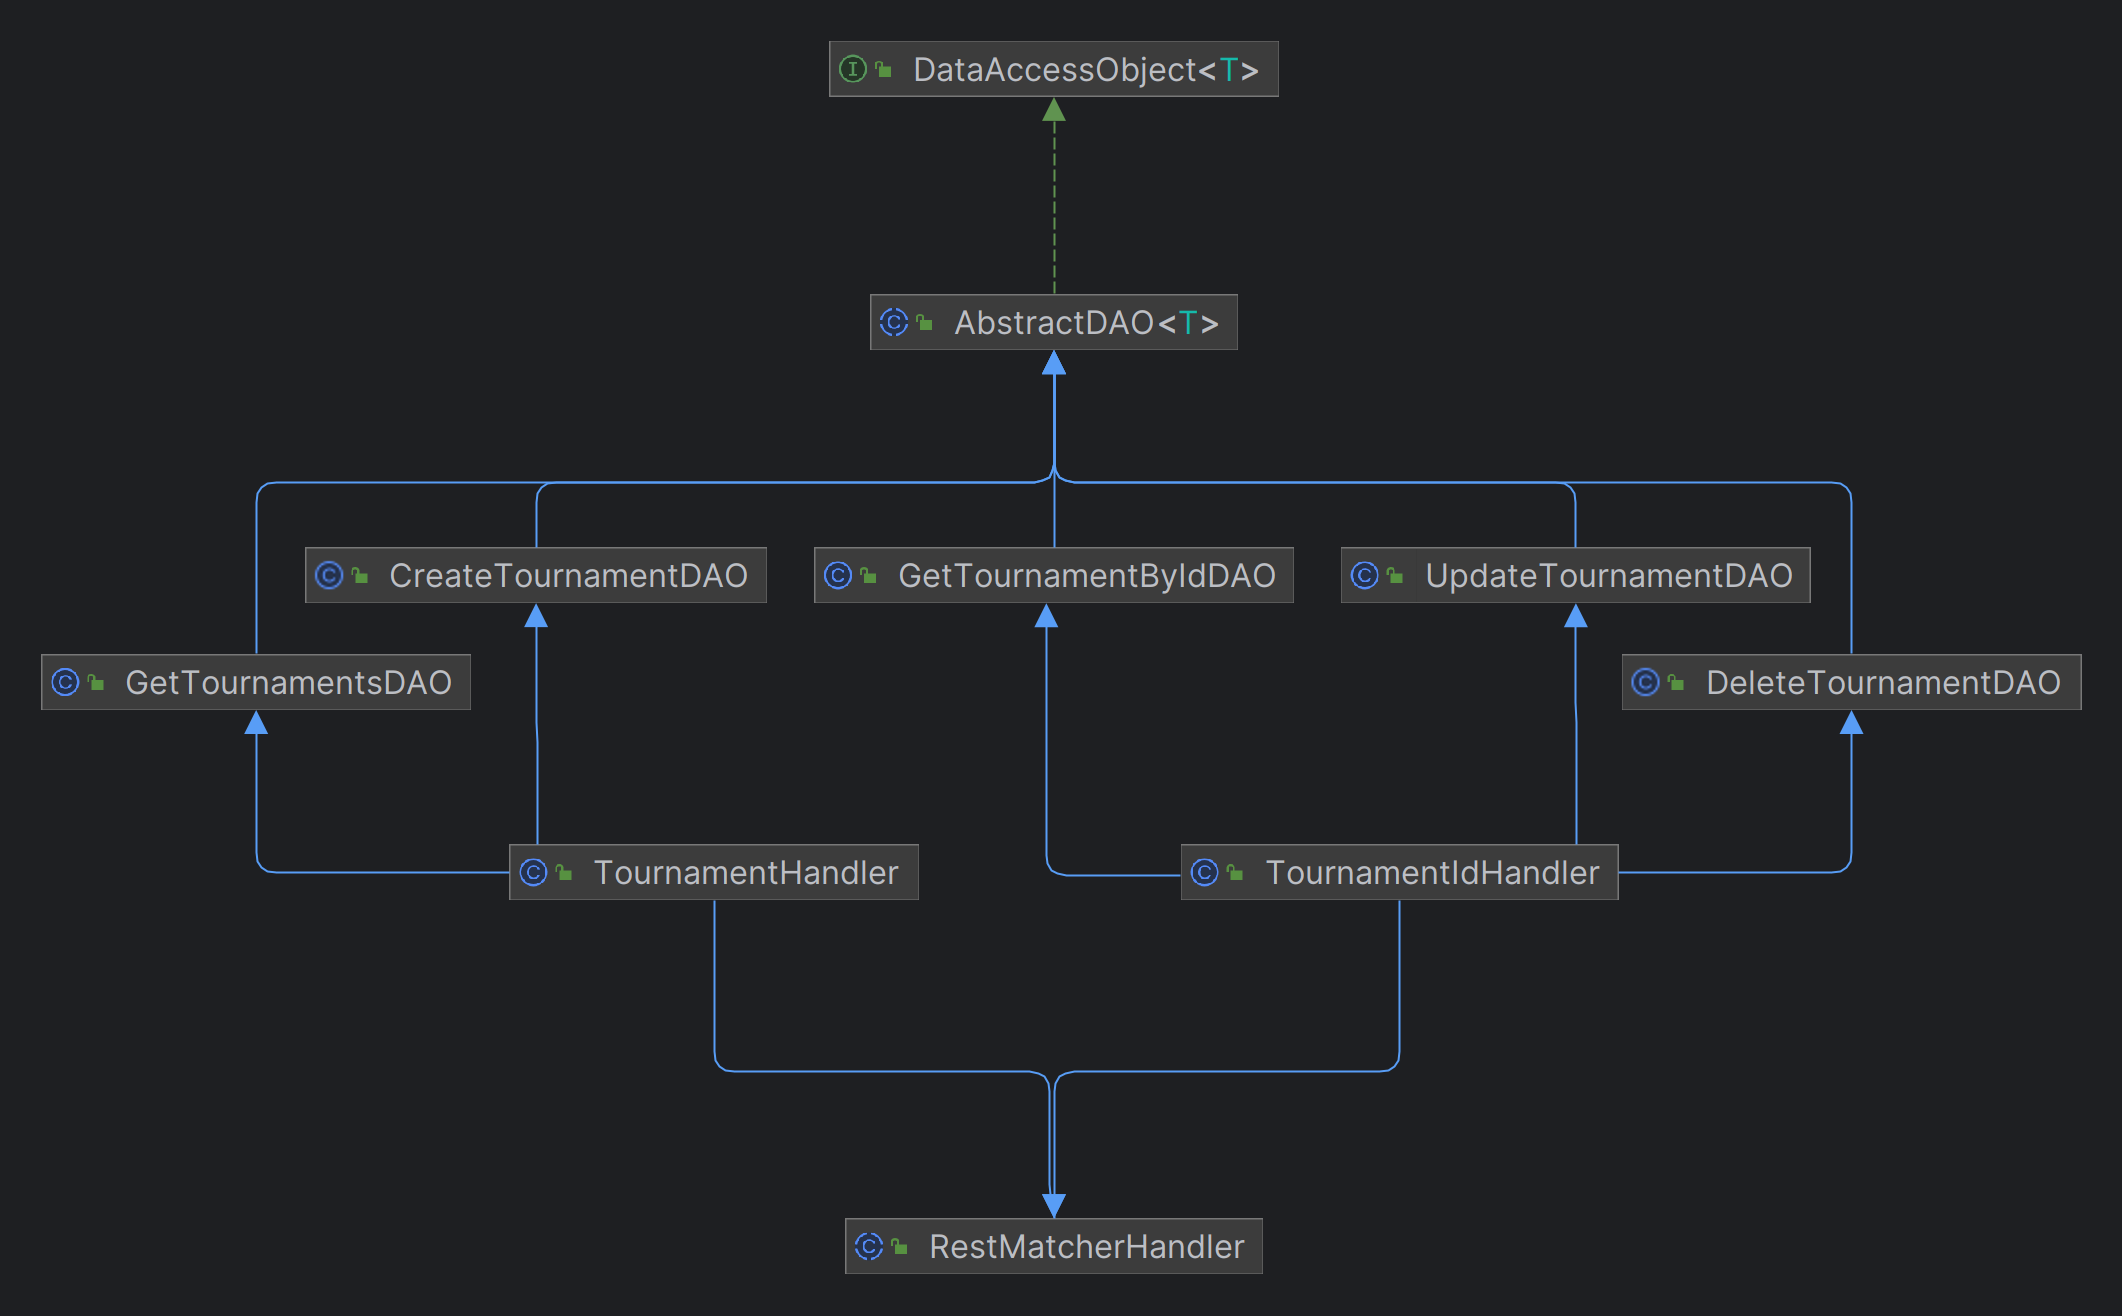
\includegraphics[]{ClassDiagram.pdf}
\textbf{IMMAGINE}

\textbf{DA MODIFICARE:}
The class diagram contains (some of) the classes used to handle six types of resources: users, tournaments, matches, teams, players and events. It is possible to observe that there is only one resource
handled by only one Servlet, that is Member. All servlets implement the doGet and doPost methods,
as sublcasses of the HttpServlet class (here omitted).
Regarding the Organizer, there are two Servlets used to handle the resource.
In particular, OrganizerServlet handles the registration of new organizers and allows to see a list of
all the organizers, together with their information. The AuthenticationServlet handles the logins in
the web application, in particular its doGet method handles the request for the logout, meanwhile
the doPost method handles the login (or in other terms, the authentication) of the users in the
application. Once the servlet has processed the request, it forwards it to the proper DAO class
(Organizer or User). Concerning the Member, the only servlet that handle this resource is UserServlet.
Such Servlet implements the doGet and doPost methods, that handle different operations. The doGet
method, through a URI request, allows to retrieve a list of all the users with their information or the
information of a single user given the phone number. The doPost method, on the other hand,
manages the registration of a new user and the upgrade of a pre-existing user’s role. Regarding the
Conferences and the conference bookings, these resources are handled through a servlet and a REST
class. The Servlet, called ConferenceReservationServlet, has a doGet method that allows to retrieve
a list of reservations given a parameter (a date or a user phone number), and a doPost method to
create a new reservation for a conference. The REST class, called ConferenceRest, manage the REST
call about conference. This class contains four methods, used to delete and insert conferences and
to retrieve a list of the attendances for all conferences or a specific one. ConferenceRest is a subclass of RestResource and is invoked from RestDispatcherServlet.
To handle the interaction with the database, we have five Data Access Objects (DAO), one for each
resource plus one to handle conference bookings: OrganizerDAO, MemberDAO, UserDAO,
ConferenceDAO and ConferenceBookDAO. Each DAO implements the methods to retrieve, insert and
update the different resources. ConferenceDAO is the only one that allows the delete operation.
Each resource is mapped into a specific data class, that has been omitted due to space reasons.
Instances of such classes are instantiated by and passed between servlets and DAOs.
